\documentclass[a4paper,10pt]{article}
\usepackage[utf8]{inputenc}
\usepackage[linguistics]{forest}
\usepackage{hyperref}
\usepackage[export]{adjustbox}
\usepackage{subcaption}
\usepackage{wrapfig}
\usepackage{fancyhdr}
\usepackage{adjustbox}



%opening
\title{Inception Document | Group 1}
\author{Kyla Kaplan & Hun Rim}
% \date{29 October 2021 - 22 November 2021}

\pagestyle{fancy}
\fancyhf{}
\rhead{November 2021}
\lhead{Group 1 | Inception Document}
\cfoot{Page \thepage}

\begin{document}
\begin{titlepage}
   \begin{center}
       \vspace*{1cm}

       \textbf{Inception Document | Group 1}

       \vspace{0.5cm}
        Topic: Computer Viruses \& Malicious Software
            
       \vspace{1.5cm}

       \textbf{Group Leaders: Kyla Kaplan \& Hun Rim}

       \vfill
            
       Approved and supervised by professor Gabriele Bavota\\
       of Software Atelier I
            
       \vspace{0.8cm}
     
       
\includegraphics[width=0.5\textwidth]{press-logo-statico-usi-orizzontale-web.png}
       
       \vspace{0.8cm}
       
       Faculty of Informatics\\
       Universit\`a della Svizzera italiana\\
       Lugano, Switzerland\\
       Date: 29 October 2021 - 22 November 2021
            
   \end{center}
\end{titlepage}

\newpage
\tableofcontents
\newpage
\section{Introduction}
The following document contains the vital information and details of our Software Atelier Group Project 1. Our group project is to develop a website consisting of a certain minimum number of pages under the topic of 'Computer Viruses \& Malware'.\\\\This 'Inception Document' contains details of our design template, planning, and scheduling of the project.\\\\The link below is the address for our Git repository:

\begin{center}\begin{verbatim}
               @atelier.inf.usi.ch:/home/bertit/group1
              \end{verbatim}
\end{center}
\section{Organization}
We have outlined 5 distinct roles in order for each member of the group to participate. Each role differs in terms of workload, responsibilities and schedule-planning. Please refer to the \hyperref[sec:Appendix]{Appendix} for tabular formats of the group organization.
\subsection*{Assigned duties \& Obligations}
 \begin{description}
 \leftskip=0.2cm\item[Team Leader:] Coordinate and present the project, while working on/ and standardising the | HTML, CSS \& Bonus Questions | while confirming their cross-compatibility and quality. Additionally, one team leader is designated to procure the Documentation in LaTeX. Must create a minimum of 1 HTML page.
\end{description}

 \begin{description}
 \leftskip=0.2cm\item[CSS Leader:] Write concise, accurate and commented CSS code that follows all necessary standardization guidelines. Must create a minimum of 1 HTML page.
\end{description}

 \begin{description}
 \leftskip=0.2cm\item[Git Leader:] Manages the Git server with its working repository, as well as, provides support to other developers when needed. Follows up on the engagement and optimizes the complexity of the project. Must also create a minimum of 1 HTML page.
\end{description}

\begin{description}
 \leftskip=0.2cm\item[Topic Leader:] Makes sure that the standardization of the development in a given time-frame is consistent and that the deadlines are met. Creates a minimum of 1 HTML page.
\end{description}

\begin{description}
 \leftskip=0.2cm\item[Team Member:] Actively participate in the creation of the website and follow all guidelines and deadlines. Must create a minimum of 4 HTML pages by the end of the project.
\end{description}

\newpage
\subsection*{Group Trees}
\begin{adjustbox}{width=\linewidth}
\begin{forest}
  [{\textbf {Group Leaders}}
    [Kyla Kaplan \& Hun Rim
      [{\textbf{Git Leader}}
        [Thomas Bertini
        ]
      ]
      [{\textbf{CSS Leaders}}
        [Nicola Fontana
        ]
        [Nicola Mazzucchelli
        ]
        ]
      [HTML Branch
      [{\textbf{Topic Leaders}}
        [{\textbf {Ilia Zeller}}
         [Alberto Sardo
         [Mattia Gianinazzi
         [Gianluca Maragliano
         [Jarod Facineroso
         [Kirustika Mohanathas
        ]]]]]]
        [{\textbf {Jeferson Morales Mariciano}}
         [Francesco Caglione
         [Paolo Deidda
         [Gianluca Ugolotti
         [Mohhammed Atwi
         [Yasemin Karakus
        ]]]]]]
        [{\textbf {Arseni Loika}}
         [Arina Shteyn
         [Alika Tsulygina
         [Phillip Krause
         [Nicolo Tafta
         [Edoardo Salvioni
        ]]]]]]
        [{\textbf {Martin Lettry}}
         [Francesco Fontana
         [Fillipo Baracca
         [Raffale Perri
         [Carson He
         [Leo Guanci
        ]]]]]]
          ]
        ]
      ]
    ]
  ]
  ]
\end{forest}
\end{adjustbox}

\vspace{3cm}
-Bonus Questions have been undefined at the given moment.

\newpage
\section{Conventions}
In order to standardize the code throughout the website development, we utilize a myriad of styling conventions to ease the process significantly and aid the user in a more coherent experience.
\vspace{1cm}
\begin{figure}[h!]
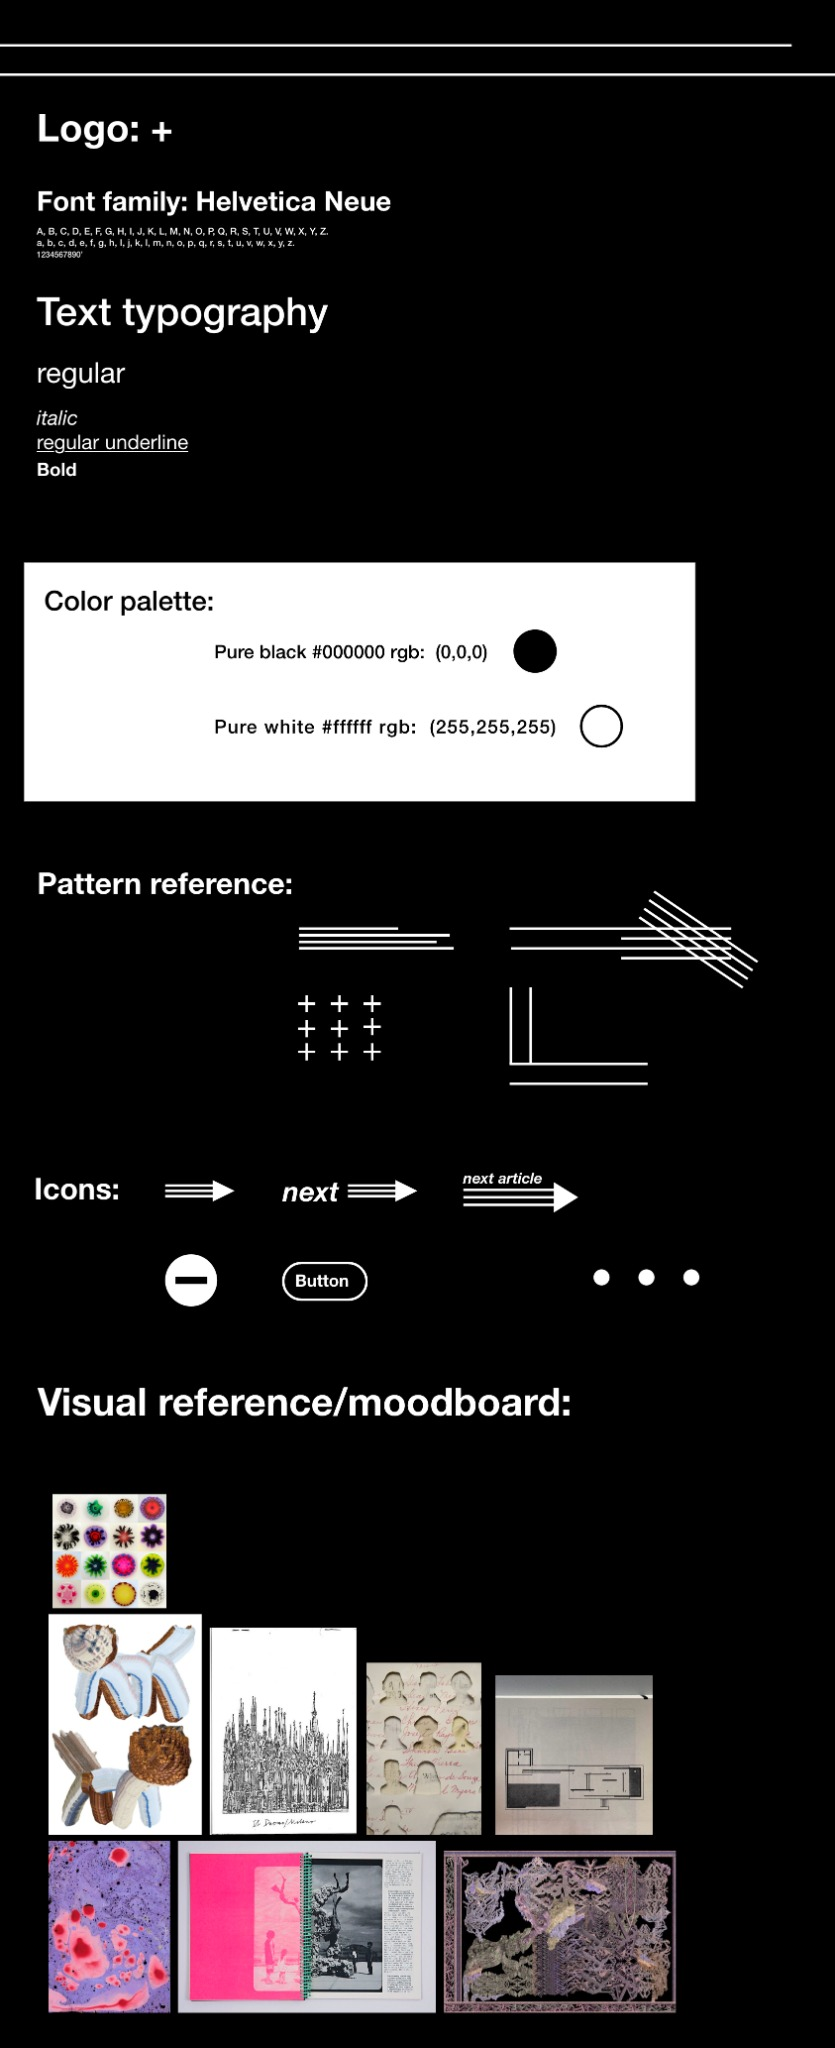
\includegraphics[height=0.52\paperheight, center]{conventions.jpeg}
\caption{Styling conventions for the CSS}
\end{figure}

\newpage
\section{Communication}
Communication during the project between all team members is of utmost importance throughout the duration of the project. Communication channels have been put in place on two seperate platforms to help aid in any discussions of topics, as wel as necessary initial introductions, etc.\\\\
Communication channels have been established via {\textbf Discord} \& {\textbf WhatsApp}.\\\\
Precedence of information is given to the main WhatsApp group 'Group 1', where all team participants are included in.\\\\
Following the main group, each 'Topic' has their own mini-group, in which at least one of the Group Leaders are present as well: 'History', 'Security', etc.\\\\
Apart from those groups, an additional one exists just for all the various leaders (i.e. Git, CSS, etc.): 'Team Leaders'.

\section{Timetable \& Due Dates}
Below is a proposed schedule for the deadlines. 

\begin{figure}[h!]
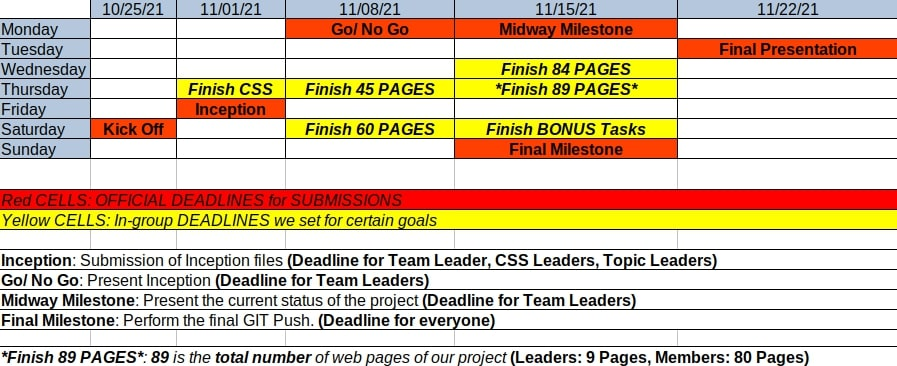
\includegraphics[width=0.9\linewidth, center]{thumbnail_timetable.jpg}
\caption{Timetable}
\end{figure}


\section{Git Utilization}
 What follows is the documentation from the GIT leader | Thomas Bertini, on how to utilize the GIT repository for the rest of the team members.\\
 
 Follow the Google Doc link: \href{https://docs.google.com/document/d/1xm-WyAb7C8v4JPY7QxbT4x-r0_QLRMDOoNHiNFWnwEI/edit?usp=drivesdk}{GIT Documentation}

\section{CSS Template}
In the following section we demonstrate the current progress of the work done by Group 1. The Git repository contains all of the files needed to render the HTML pages shown below. There are remaining plans to refine the code and resolve some minor issues and bugs, as well as, work on the overall feel of the each individual page. Please keep in mind that the renders shown below are for demonstration purposes.
\begin{center} 
{\textit{Members currently working on the CSS are as previously mentioned:\\
Nicola F., Nicola M. }}
\end{center}

\begin{figure}[p]

\includegraphics[height=0.52\paperheight, center]{homepage_page.jpeg}
\caption{Proposed Homepage}
\end{figure}

\begin{figure}[p]
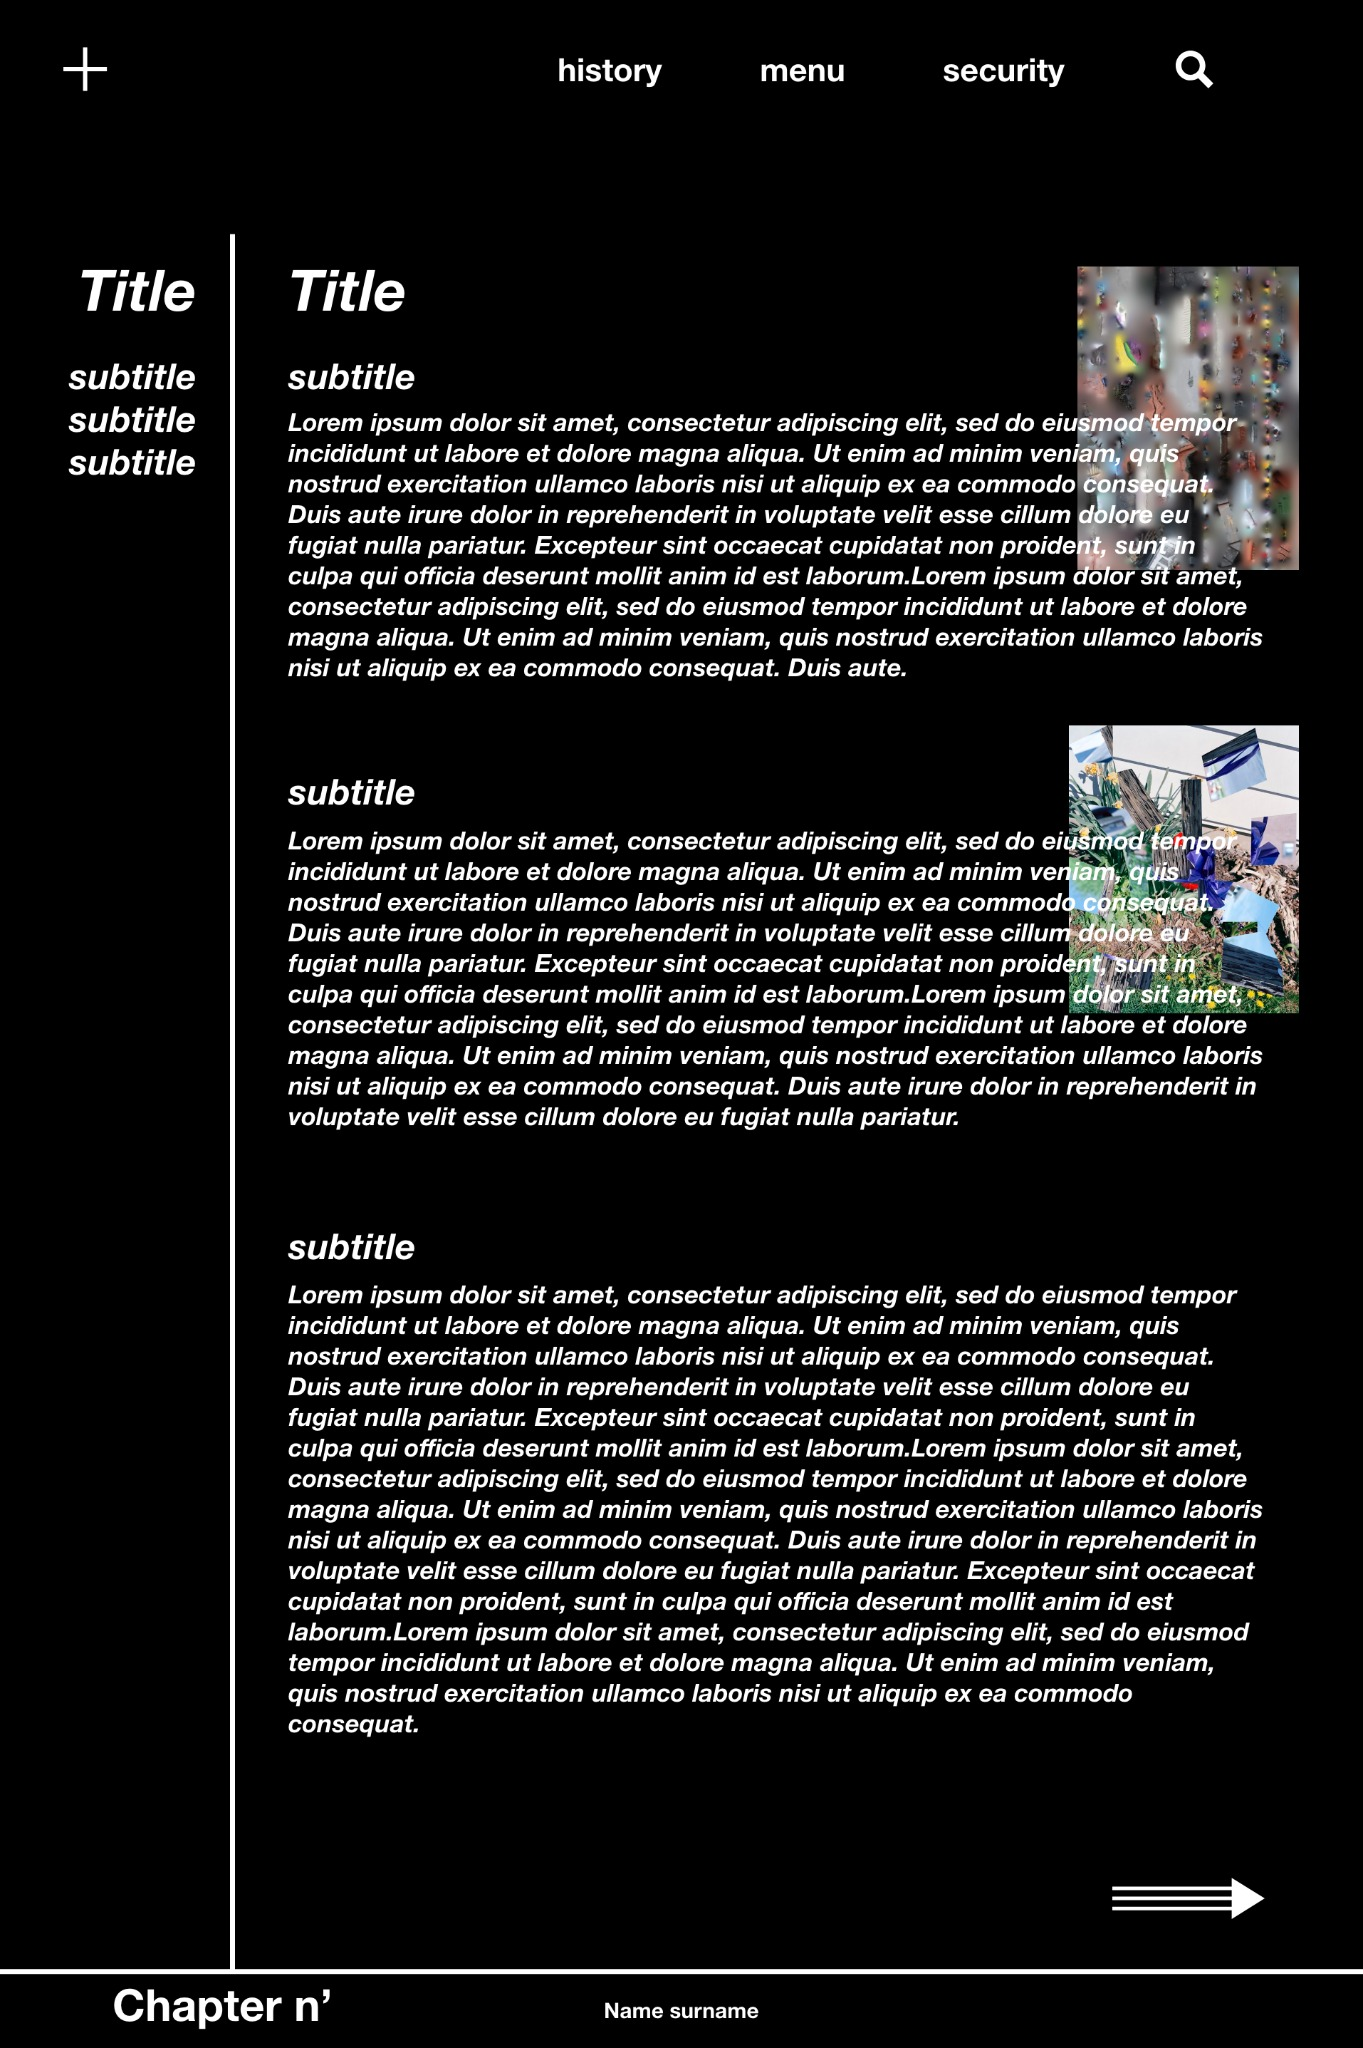
\includegraphics[height=0.52\paperheight, center]{virus_article.jpeg}
\caption{Virus Section Article Page}
\end{figure}

\begin{figure}[p]
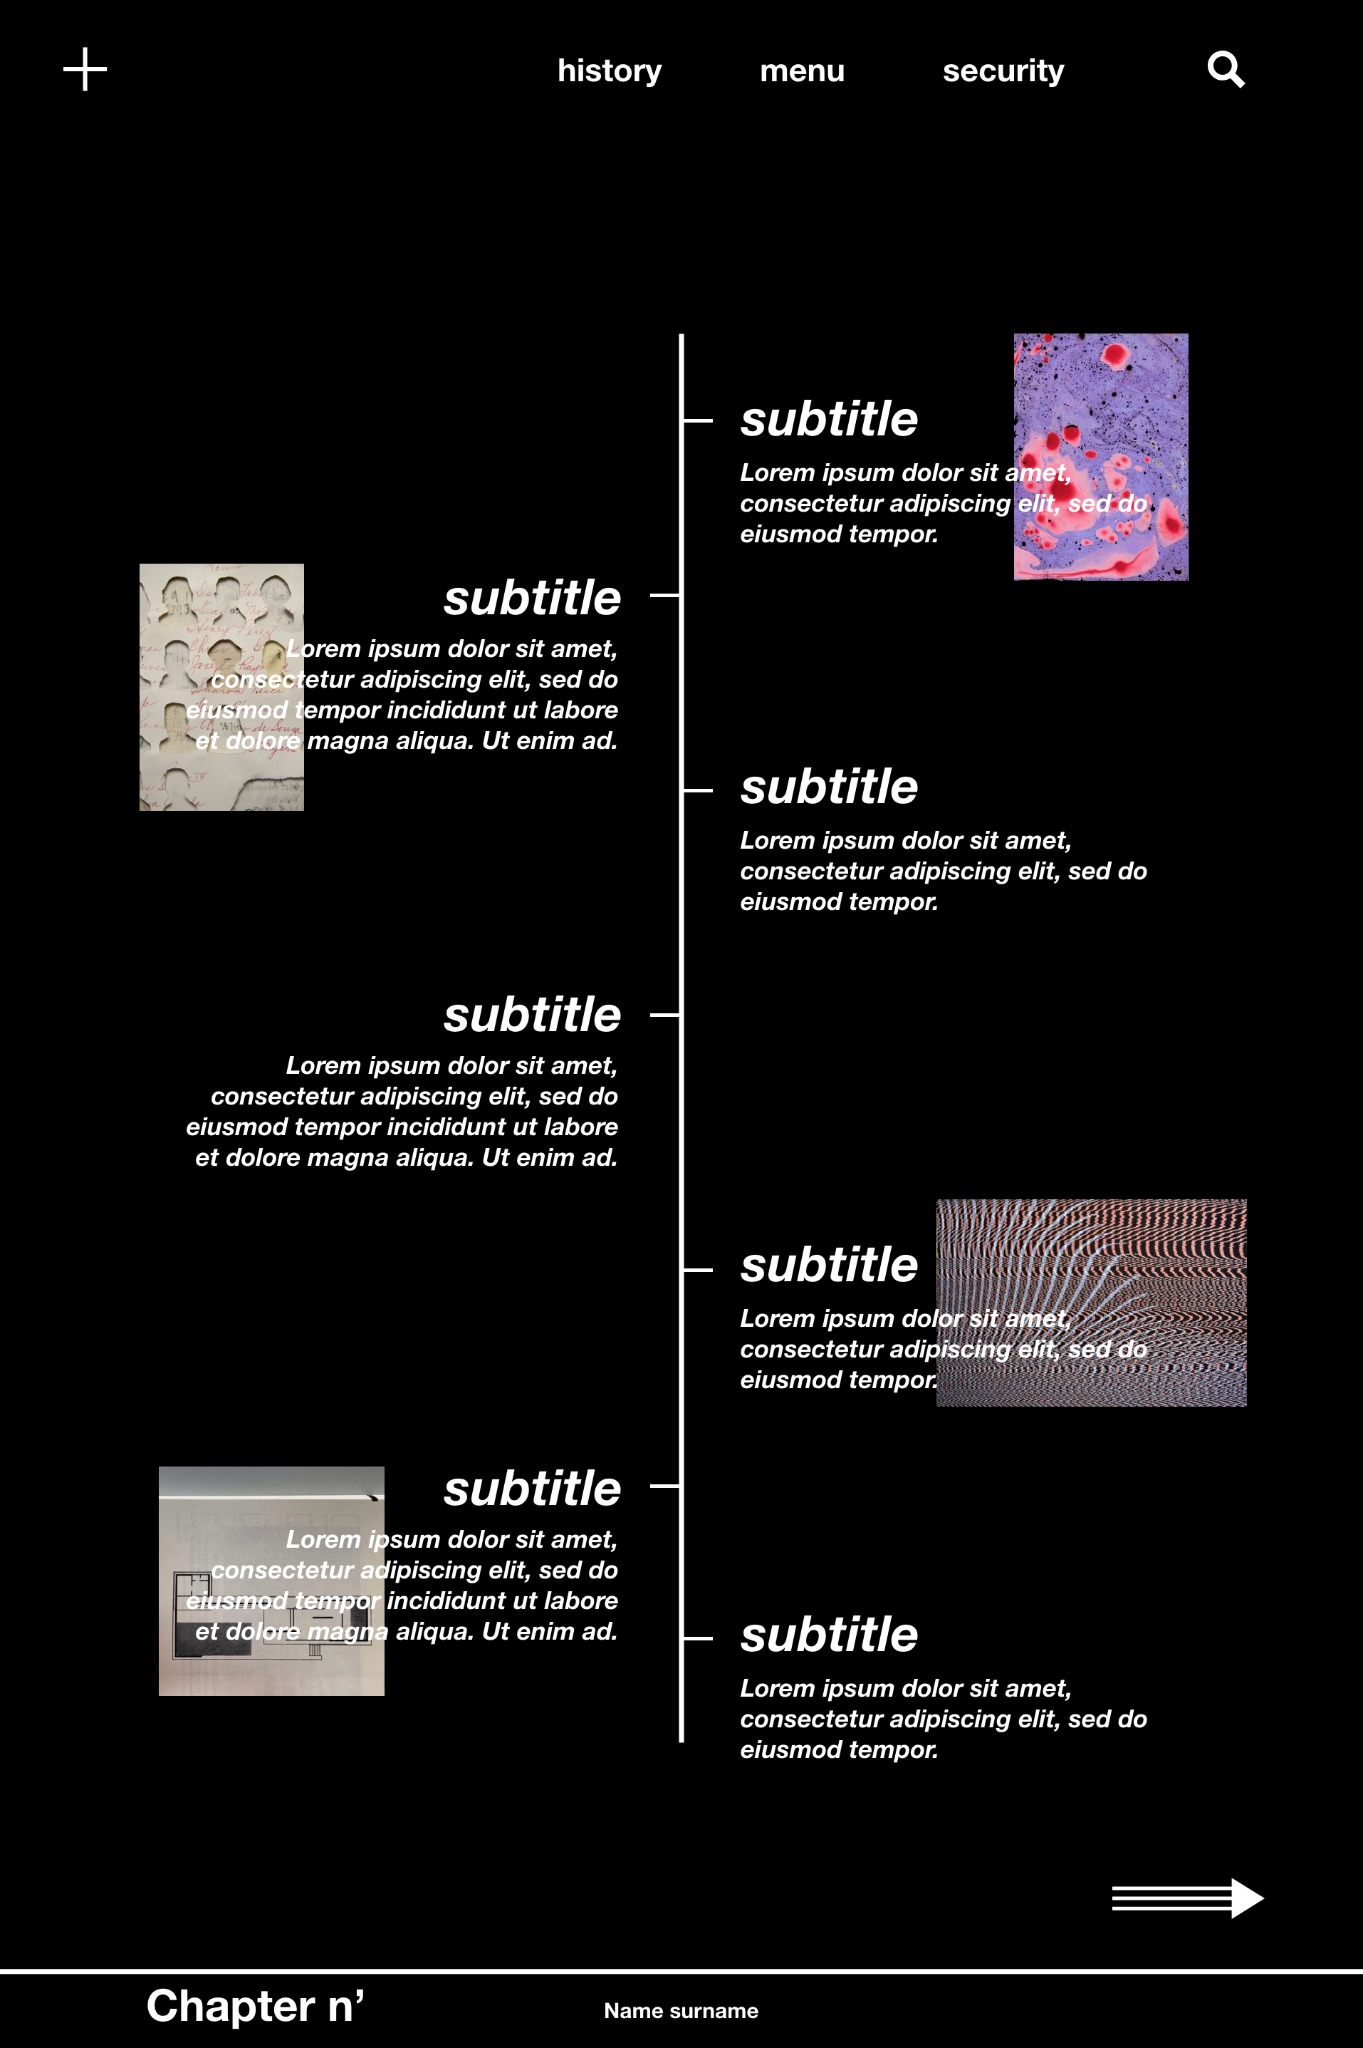
\includegraphics[height=0.52\paperheight, center]{history_timeline_article_page.jpeg}
\caption{History Section Timeline Page}
\end{figure}

\begin{figure}[p]
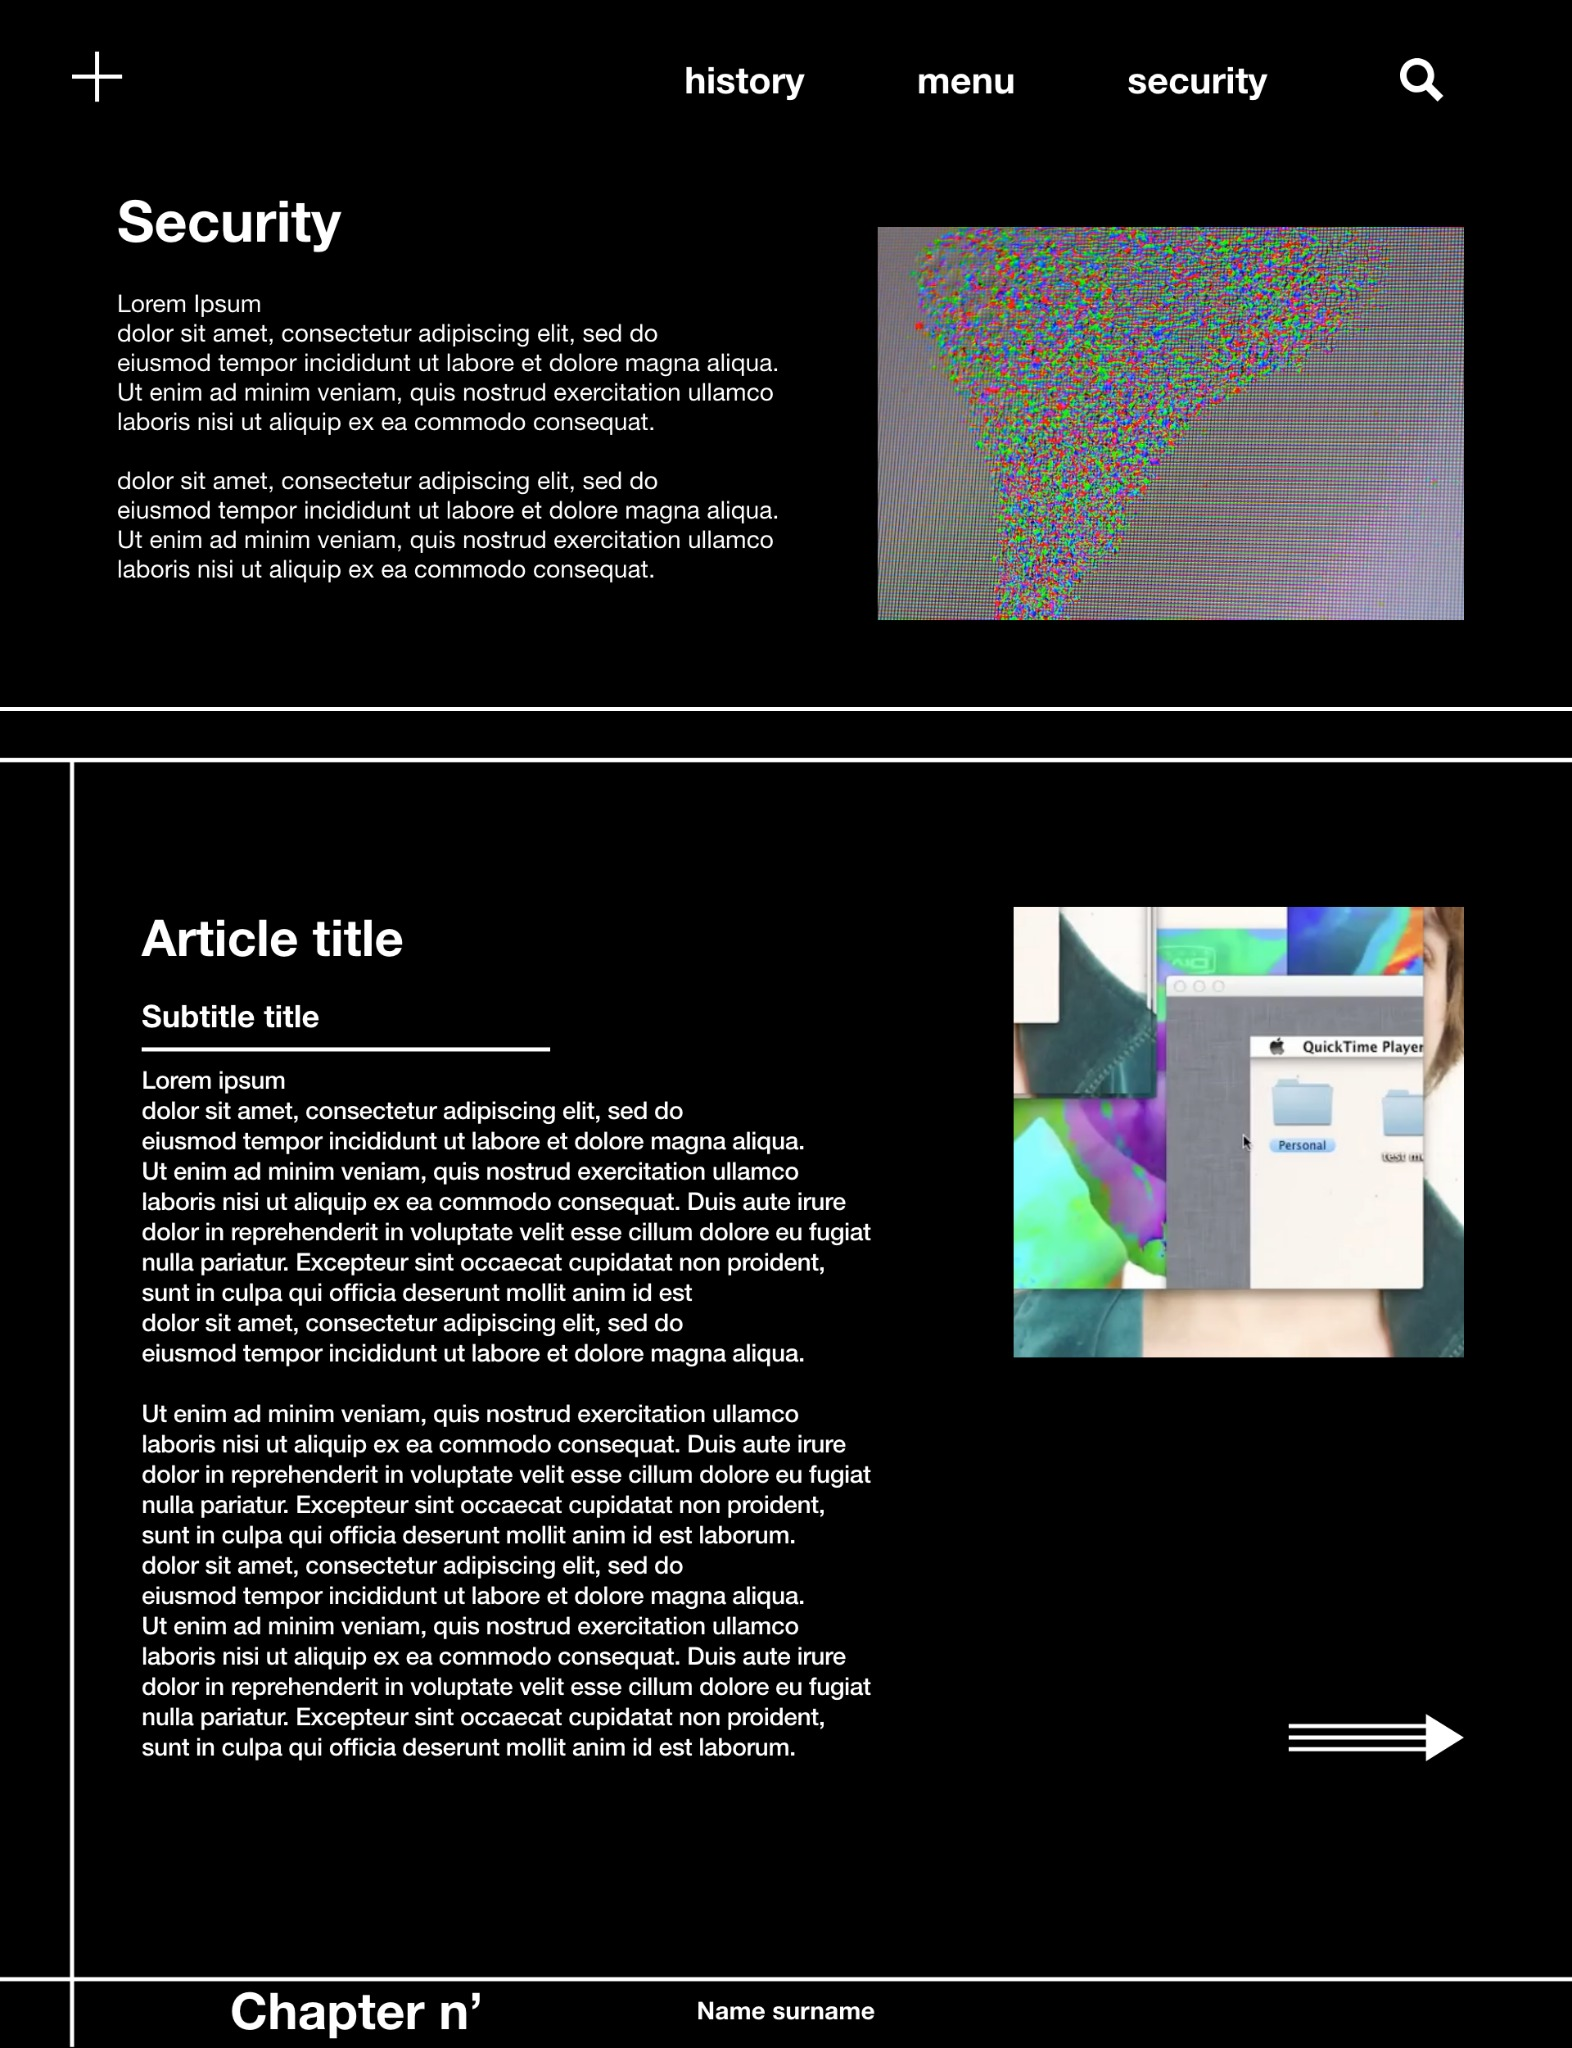
\includegraphics[height=0.52\paperheight, center]{security_article_page.jpeg}
\caption{Security Section Article Page}
\end{figure}

\begin{figure}[p]
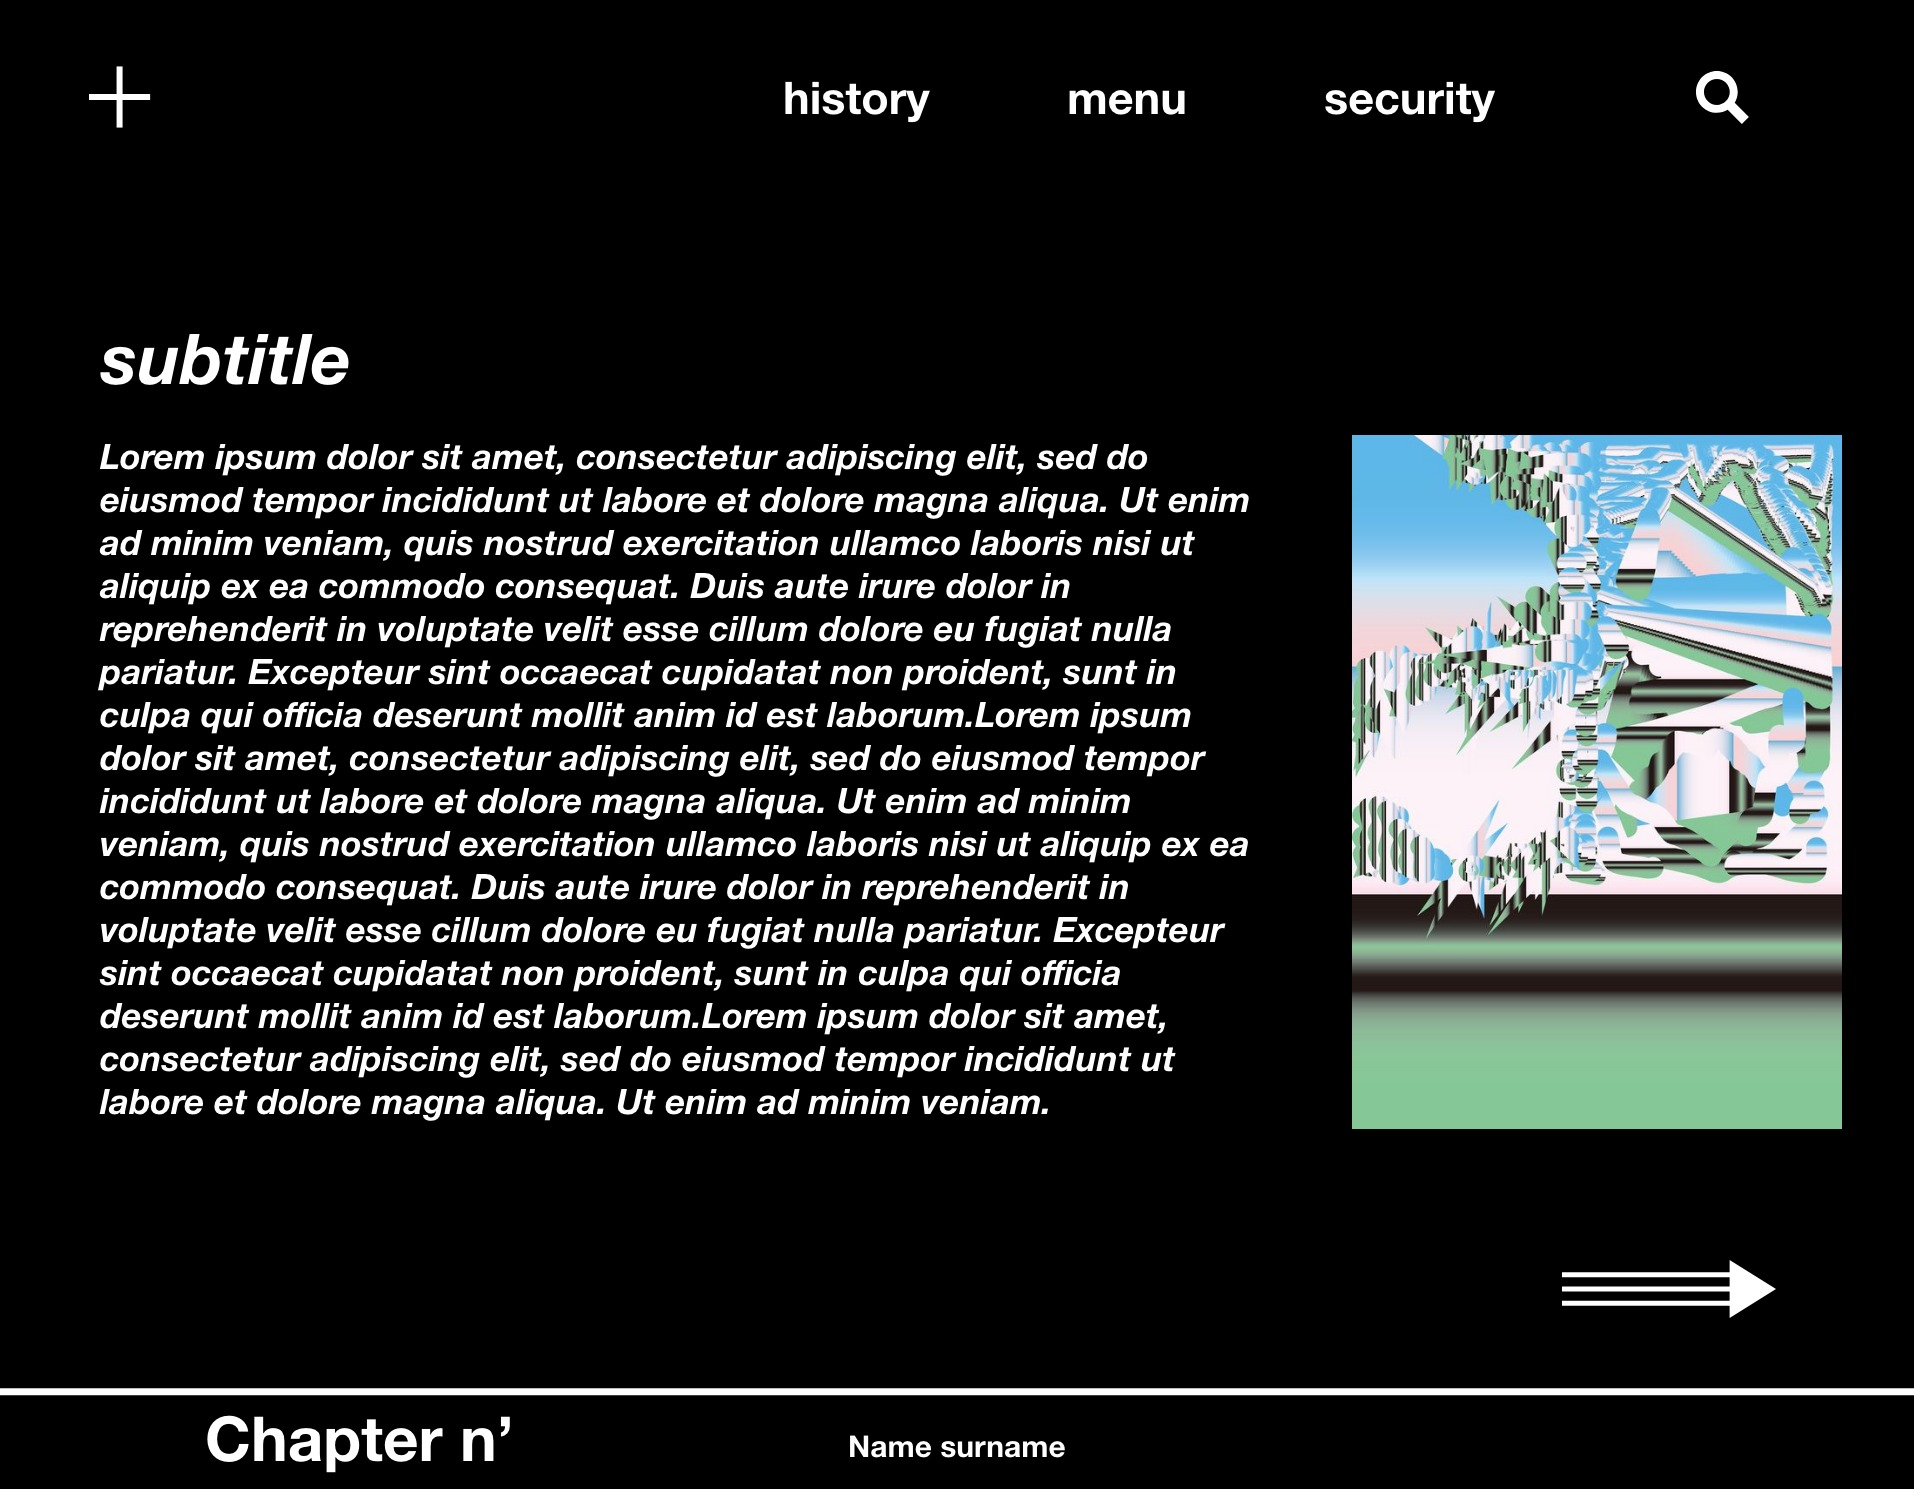
\includegraphics[height=0.52\paperheight, center]{malware_page.jpeg}
\caption{Malware Article Page}
\end{figure}

\begin{figure}[p]
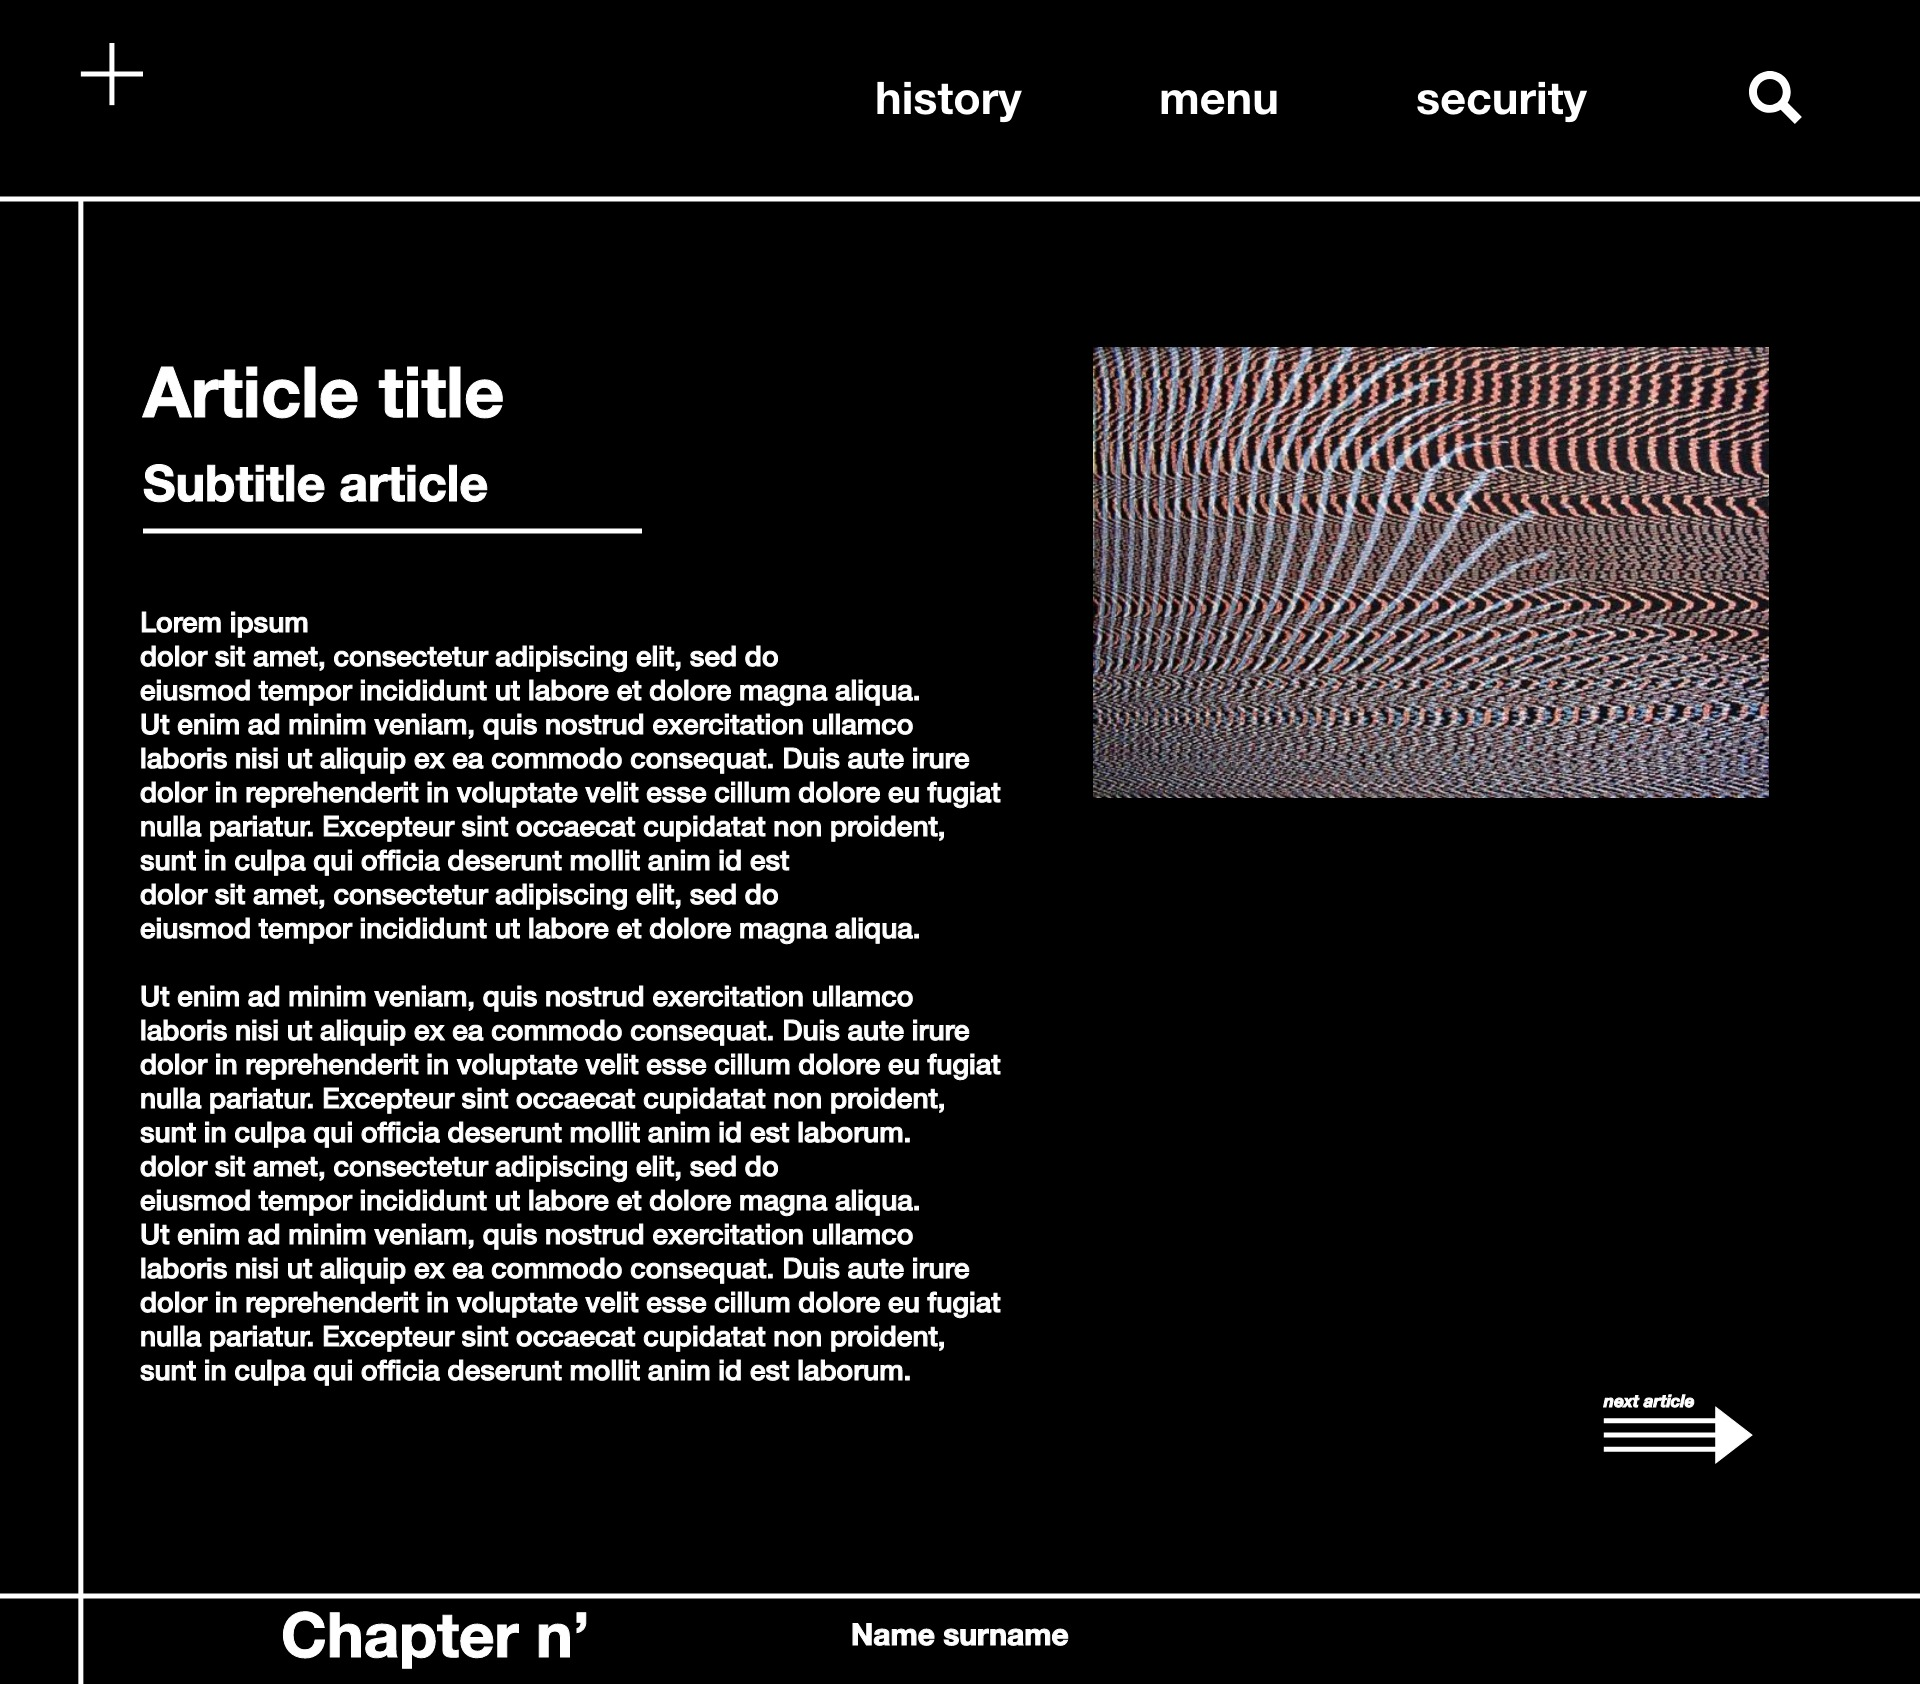
\includegraphics[height=0.52\paperheight, center]{alternative_malware_page.jpeg}
\caption{Alternative Malware Article Page}
\end{figure}

\begin{figure}[p]
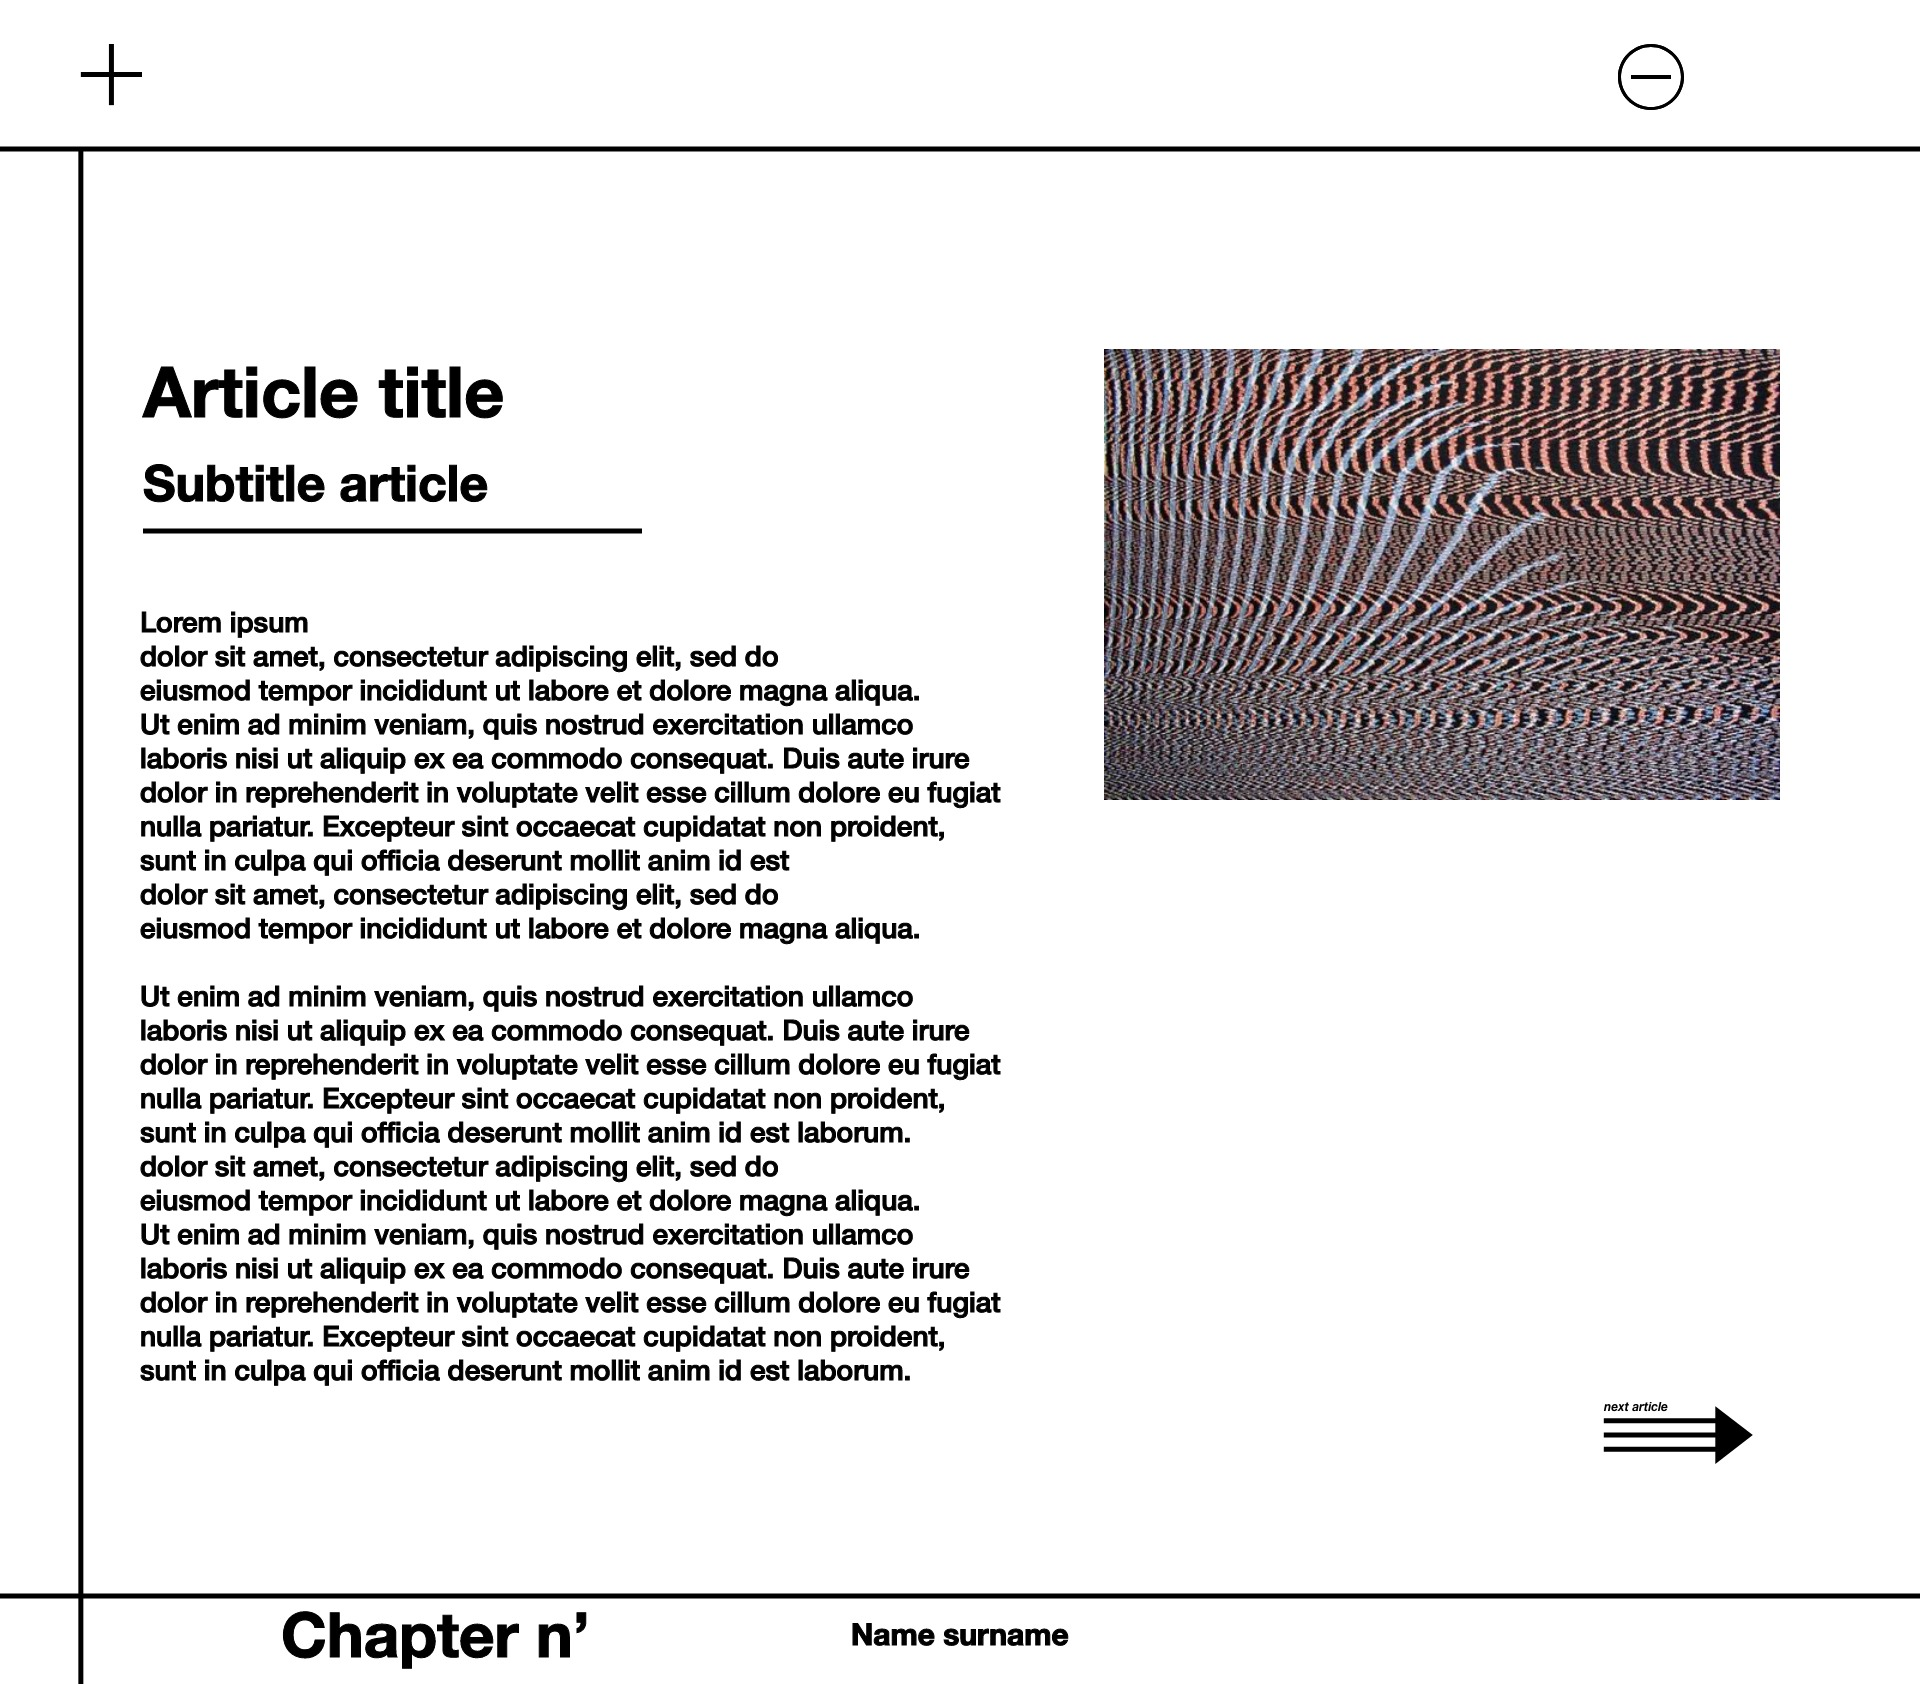
\includegraphics[height=0.52\paperheight, center]{lightmode_articletitle.jpeg}
\caption{Light mode of the Article Page}
\end{figure}

\begin{figure}[p]
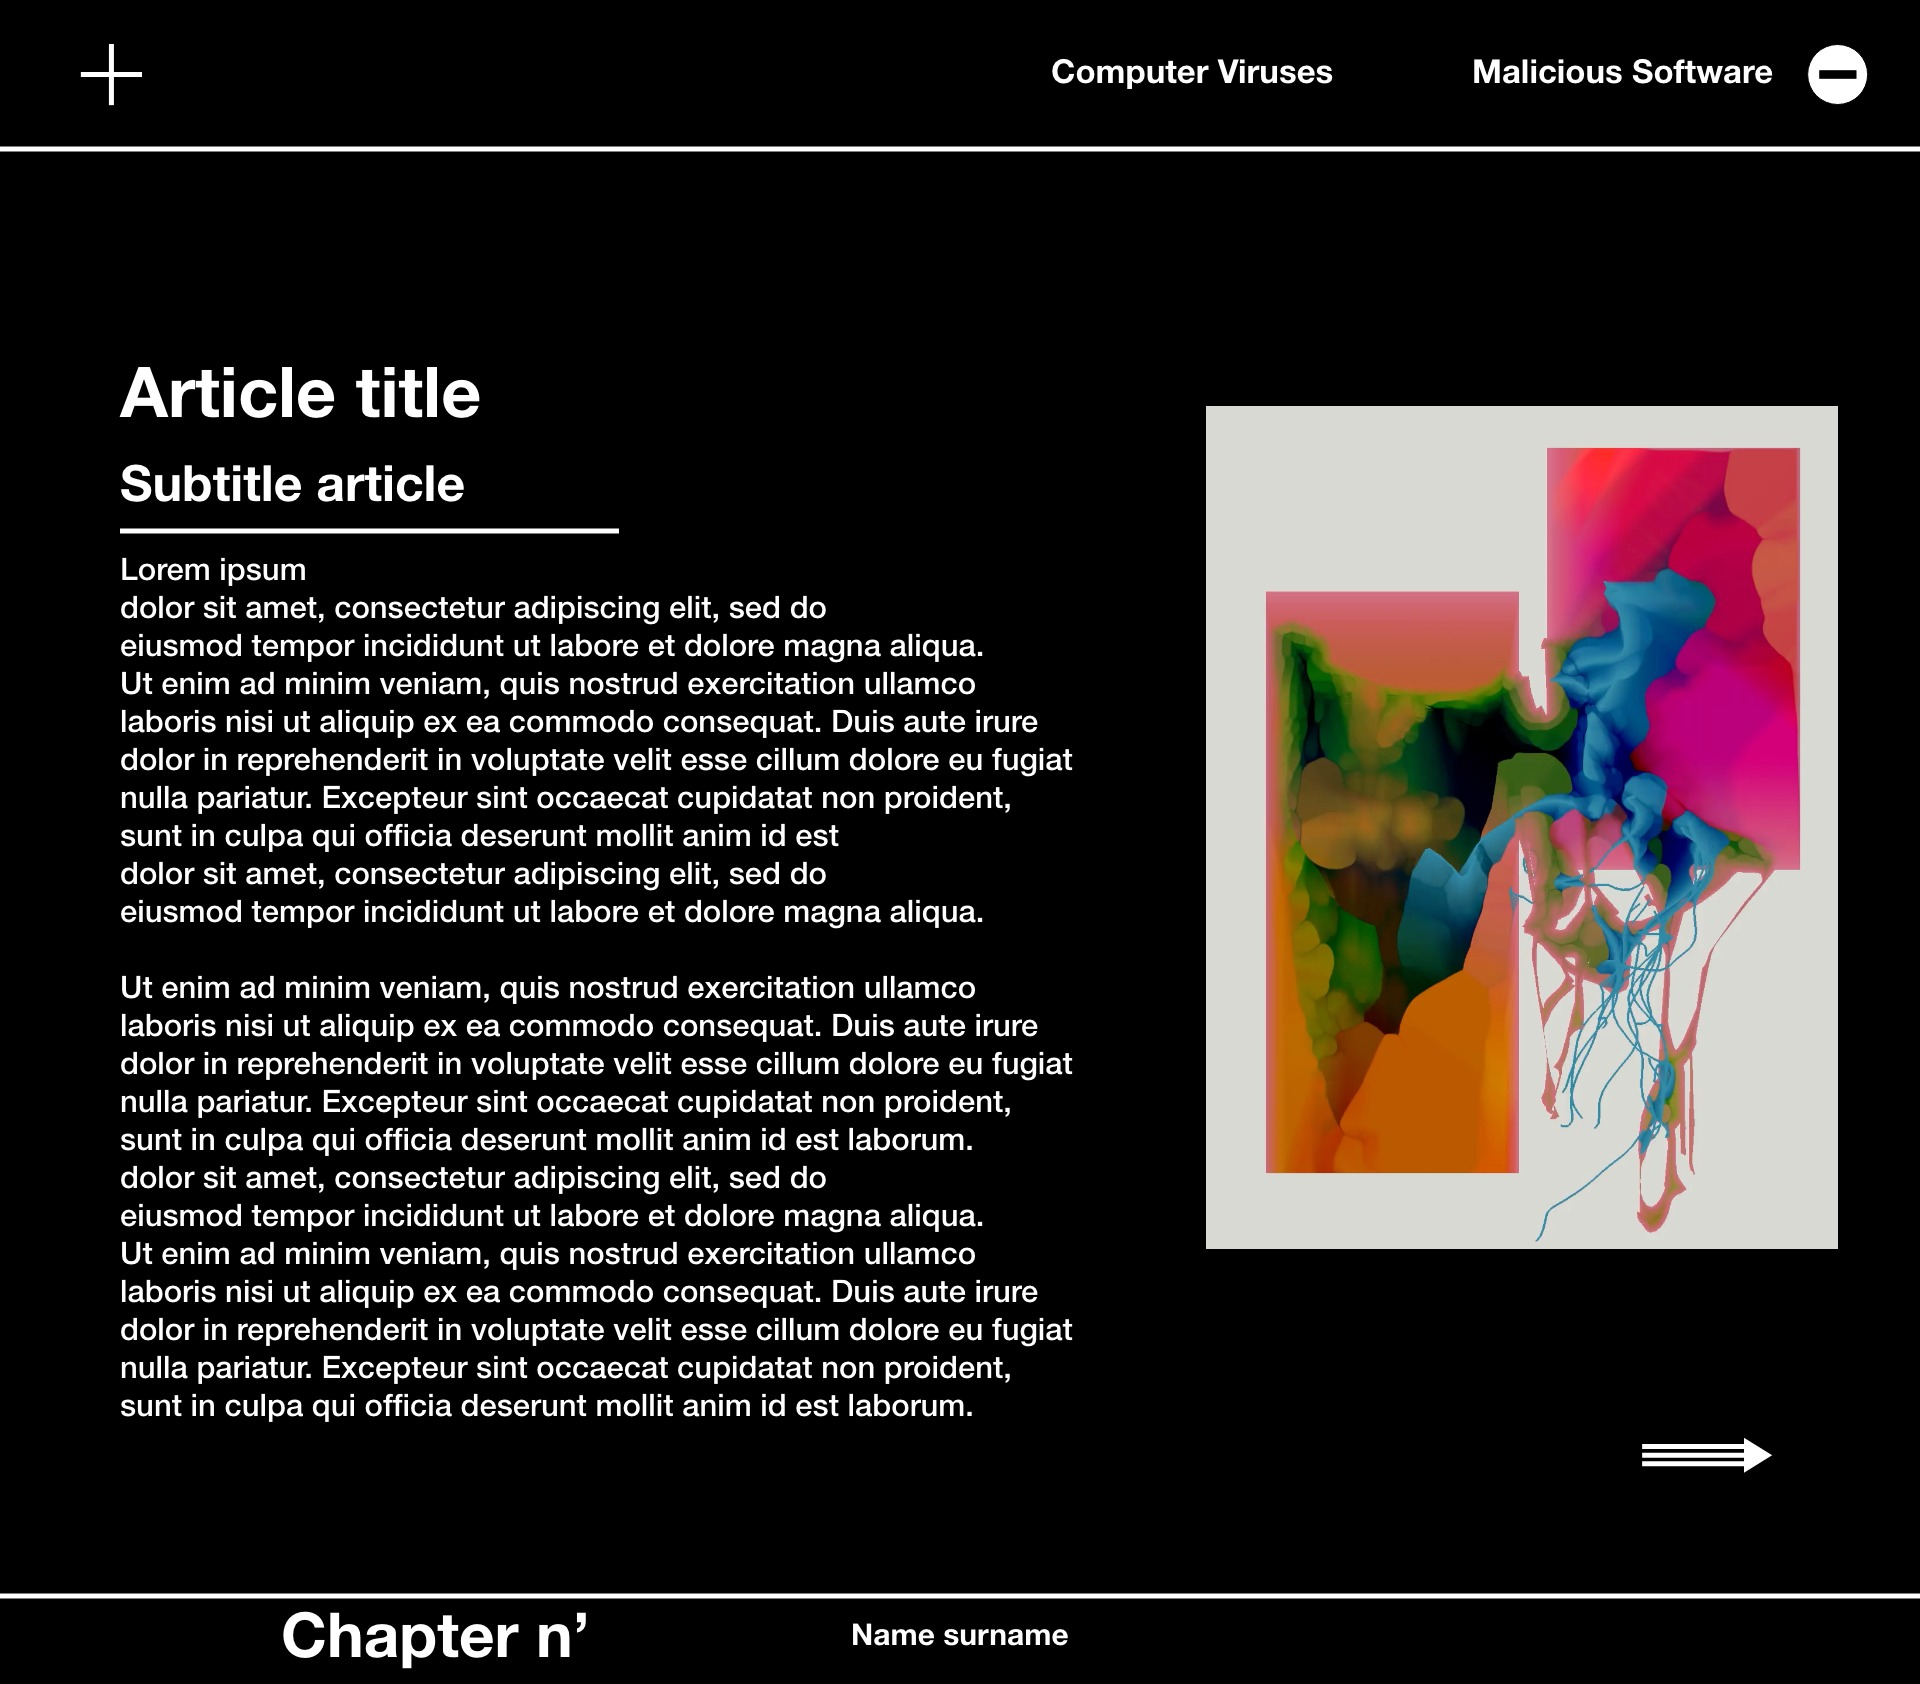
\includegraphics[height=0.52\paperheight, center]{darkmode_articletitle.jpeg}
\caption{Dark mode of the Article Page}
\end{figure}




\newpage
\section{Appendix}
\label{sec:Appendix}
\subsection*{List of Participants}
\begin{figure}[h!]
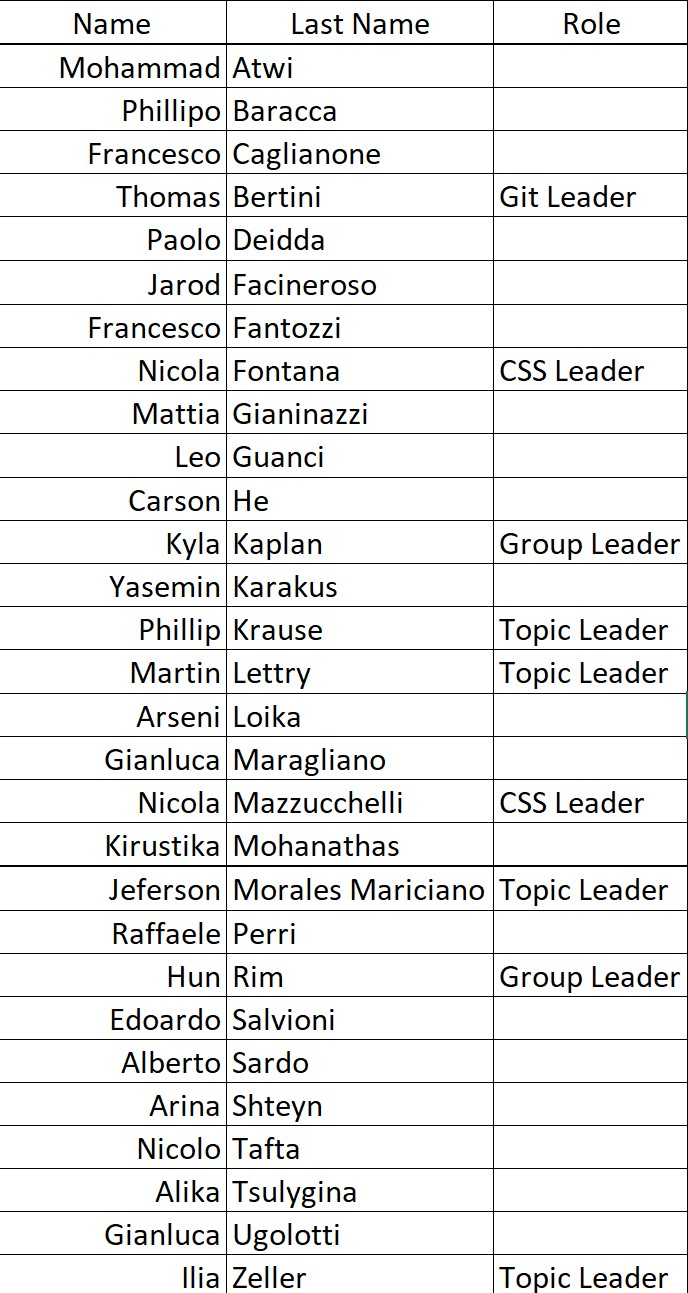
\includegraphics[height=0.52\paperheight, center]{Group_Participants.jpg}
\caption{List of Group Participants}
\end{figure}

\newpage
\vspace{1cm}
\subsection*{Organization of Topic Participants}
\begin{figure}[h!]
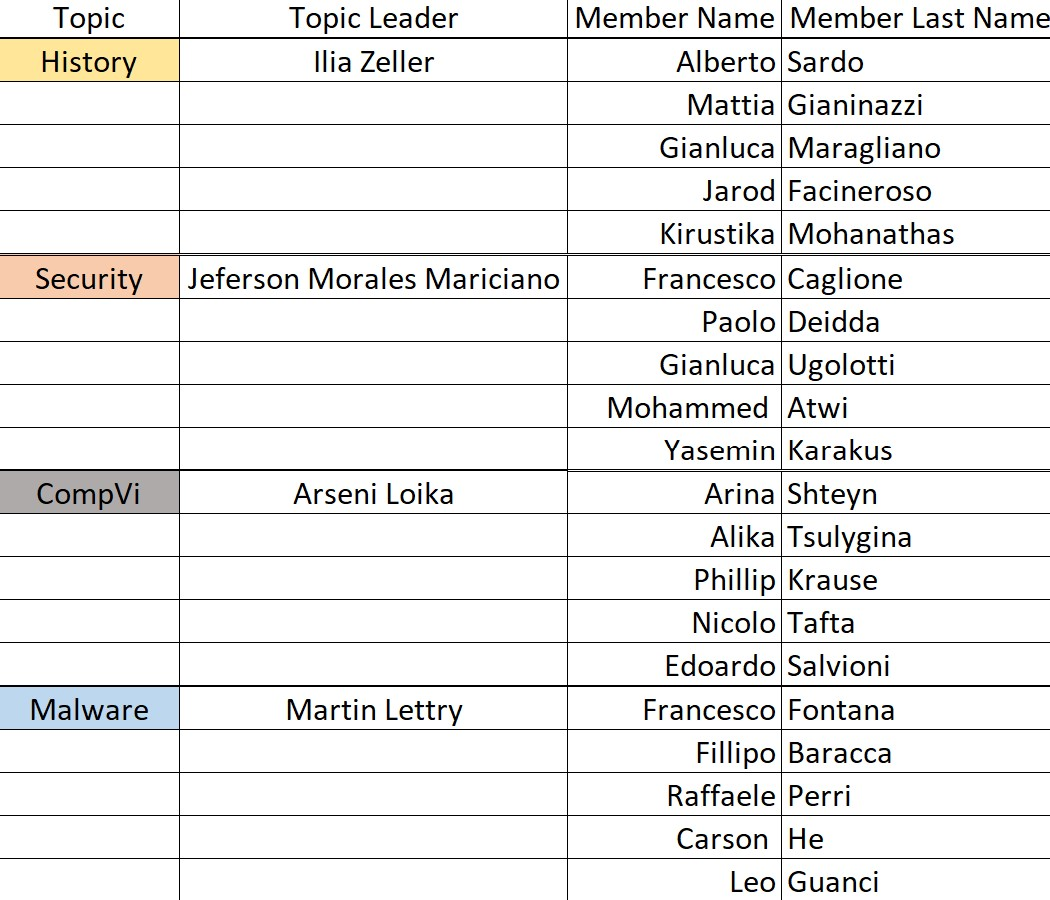
\includegraphics[height=0.52\paperheight, center]{subtopic_members.jpg}
\caption{List of Topic Participants}
\end{figure}


\end{document}
